\chapter{Grover's algorithm}

[TODO: Cite: https://qiskit.org/textbook/ch-algorithms/grover.html]

Grover's search algorithm is a quantum algorithm framework, that takes a user-defined solution verifier algorithm (the oracle) and turns it into a $\Theta(\sqrt{N})$ solver. This provides a quadratic speedup over the classical brute force equivalent.

Many sources call this a database search algorithm, since in Grover's original paper it was described as such. However, the 'database' here is an abstract entity, that represents the entire domain of the problem, while the so-called 'marked' elements are the correct solutions in this domain, for which the oracle would return a 'YES' answer. Using the terms 'problem domain' instead of 'database', 'verifier algorithm' insead of 'oracle' and 'solutions' instead of 'marked elements' makes Grover's importance and connection to the P versus NP problem clearer and the details of the algorithm easier to understand.

Another common description of Grover's search algorithm is that it can solve 'unstructured search problems'. What they mean by this is that the algorithm doesn't construct a solution by iterating over partial solutions or improving a non-solution step-by-step. Constrast this with for example how Prim's minimum spanning tree algorithm iterates on partial solutions by connecting the remaining vertices of the graph one at a time. This requires knowledge of the graph and knowledge of how to build a minimal spanning tree one vertex at a time.

Grover doesn't need to know the structure of the original problem, the relationship between partial solutions or how to improve non-solutions. It only needs to know how to verify a solution. It starts by taking all of the entities from the problem's domain with uniform distribution.

\begin{figure}[H]
    \centering
    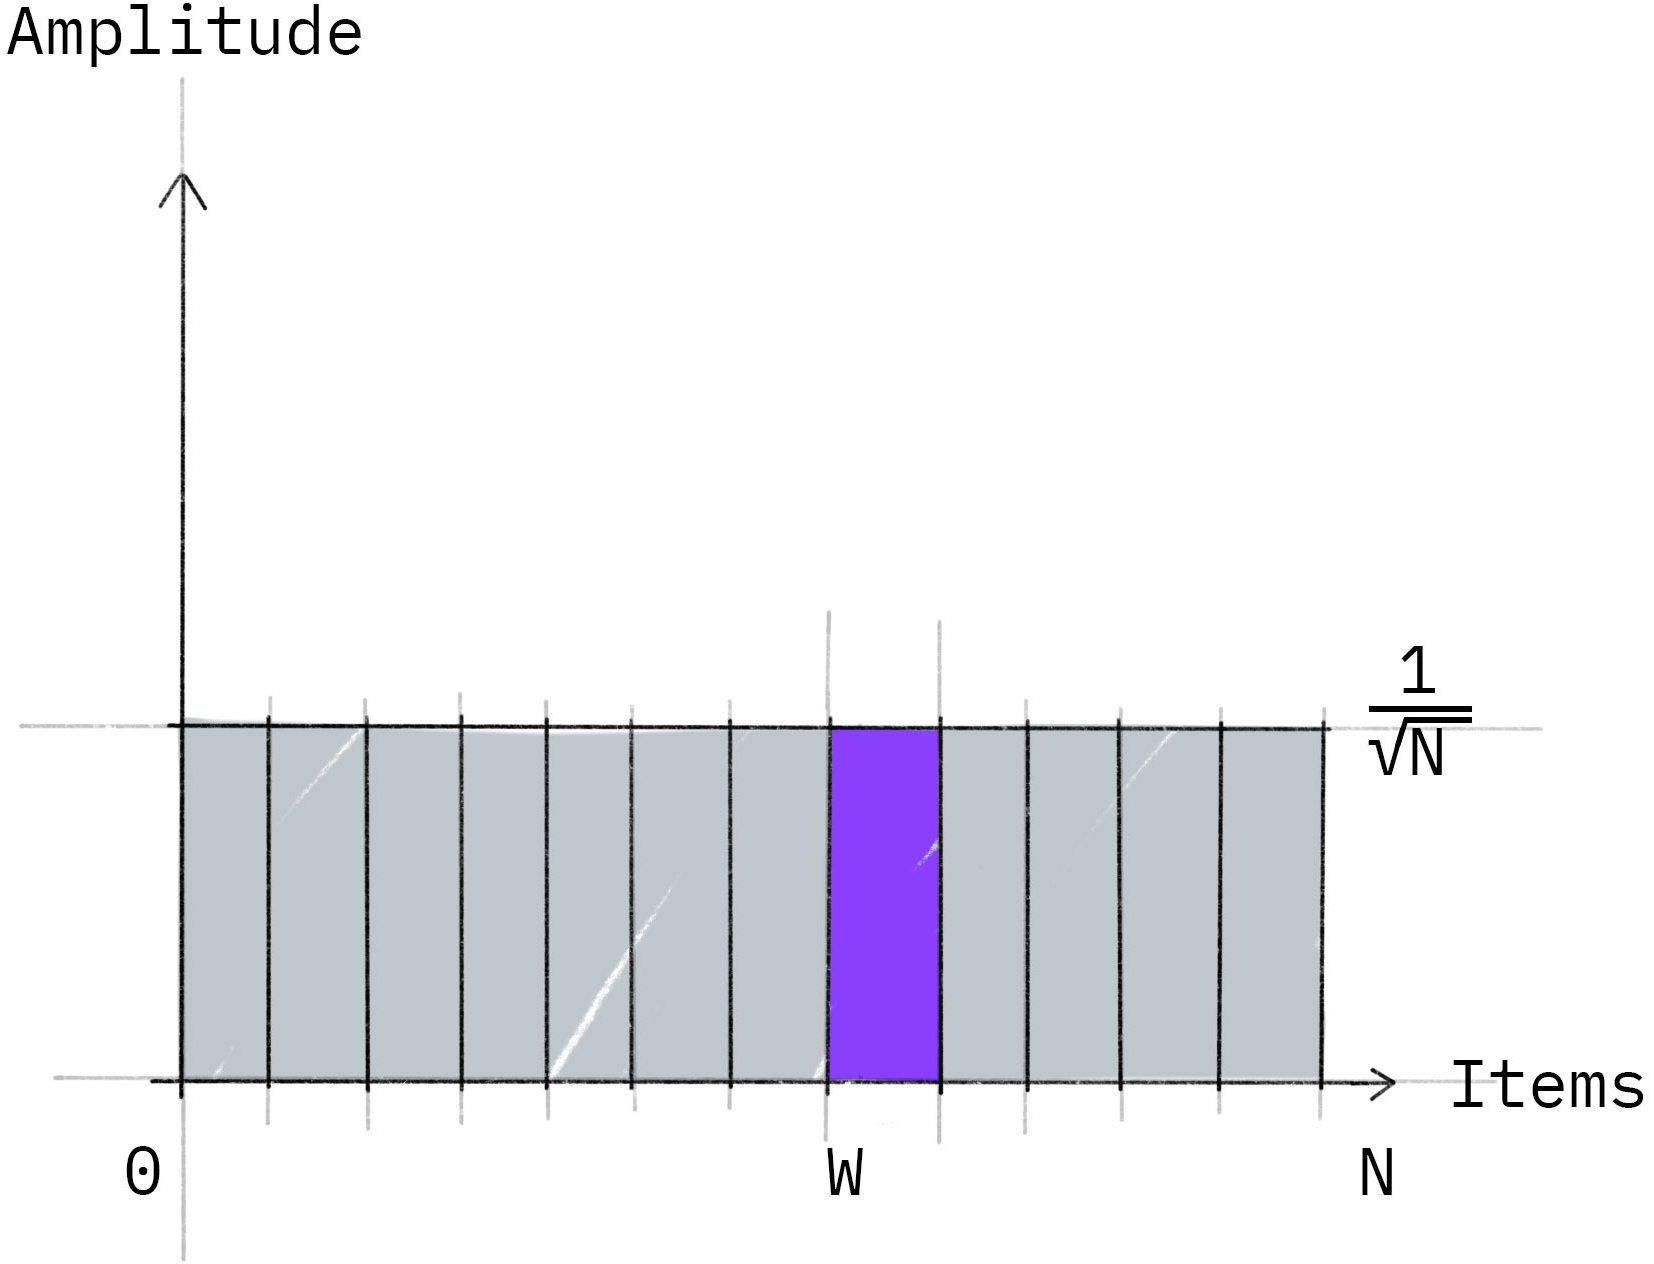
\includegraphics[width=0.5\linewidth]{content/assets/03_grovers_algorithm/grover_uniform.jpg}
    \caption{Grover starts out with the uniform distribution}
    \label{fig:grover_uniform}
\end{figure}

Then, it uses the verifier algorithm to manipulate their probabilities until the correct entities' probabilities are very high, while the incorrect entities' probabilities are very low.

\begin{figure}[H]
    \centering
    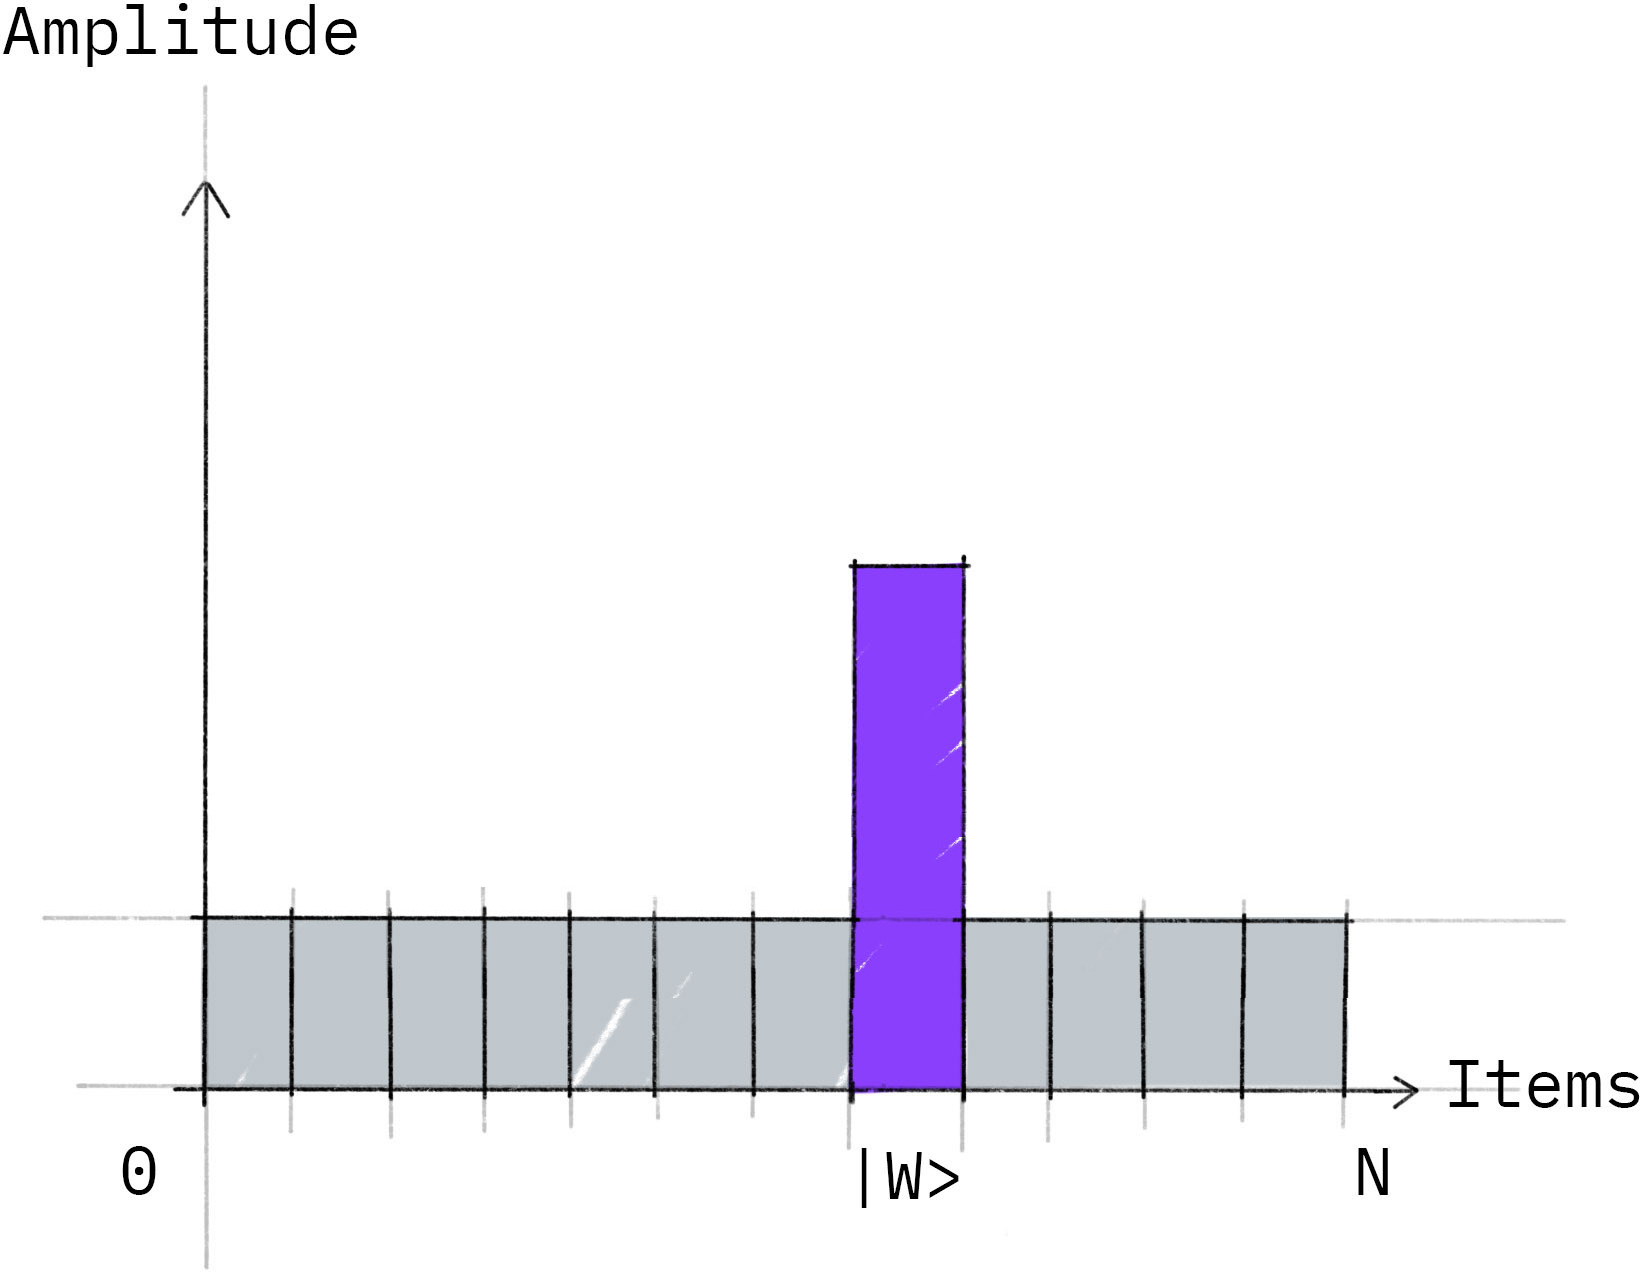
\includegraphics[width=0.5\linewidth]{content/assets/03_grovers_algorithm/grover_final.jpg}
    \caption{Grover starts out with the uniform distribution}
    \label{fig:grover_uniform}
\end{figure}

Finally, it samples from this probability distribution, which results in a correct solution entity with a high chance.

Working with a probability distribution over an exponentially large set of entities is only possible in a memory-efficient way on a quantum computer, thanks to the quantum physical nature of qubits. A register of classical bits can only represent a single entity, we would need separate registers to represent a set and we can only operate on the entire set in a linear fashion, one register at a time. In contrast, a register of quantum bits, or 'qubits' itself can represent a set of entities from the domain using the quantum physical phenomenon of superposition.

When we read this register's contants, we can only sample a single element from the probability distribution, we cannot iterate all.

The probability distribution over this set and some of the probability distributions (especially the ones that have zeros in them) are only possible because of entanglement.

The manipulation of these probabilities happens using quantum operators or gates, which are the basis of all quantum algorithms on gated general-purpose quantum computers.

